\documentclass{assignment}
\usepackage{listings}
\usepackage[indonesian]{babel}
\usepackage{xcolor}
\usepackage{caption}
\usepackage{amsmath,amssymb,amsfonts}
\usepackage{mdframed}
\usepackage{hyperref}
\usepackage{graphicx}
\usepackage{geometry}
\usepackage{float}

% Document Configurations
\captionsetup[figure]{name={Gambar},labelsep=period}
\coursetitle{Pengolahan Citra Digital}
\courselabel{}
\exercisesheet{Citra Gambar Bergerak (GIF)}{}
\student{Helmy Luqmanulhakim - 22051204014}
\semester{Genap 2023/2024}
\school{S1 Teknik Informatika}
\university{Universitas Negeri Surabaya}
\date{24 Februari 2024}
\newcommand\tab[1][0.5cm]{\hspace*{#1}}

\geometry{a4paper, left=3cm, right=2cm, top=3cm, bottom=3cm}

\lstdefinestyle{code}{
    basicstyle=\ttfamily,
    numberstyle=\tiny,
    numbersep=5pt,
    tabsize=4,
    extendedchars=true,
    breaklines=true,
    keywordstyle=\color[rgb]{0,0,1},
    identifierstyle=\color[rgb]{0.2,0.2,0.2},
    commentstyle=\color[rgb]{0.25,0.5,0.37},
    stringstyle=\color[rgb]{0.16,0.5,0.16},
    showspaces=false,
    showtabs=false,
    xleftmargin=1.5em,
    xrightmargin=0.5em,
    framexleftmargin=1em,
}



% Pages
\begin{document}
\section*{Pendahuluan}
\tab Dalam era yang semakin terkoneksi dan dipenuhi dengan konten visual, kemampuan untuk menciptakan gambar bergerak menjadi keahlian yang sangat dicari. Pengolahan citra digital menjadi landasan utama dalam menciptakan karya visual yang memukau. Praktikum ini akan membahas salah satu aspek yang paling menarik dari pengolahan citra: pembuatan gambar bergerak dalam format GIF, dengan menggunakan bahasa pemrograman Python dan perpustakaan PIL (\textit{Python Imaging Library}).


\section*{Tujuan}
\tab Praktikum ini bertujuan untuk memahami konsep dasar pembuatan gambar bergerak dalam format GIF. Dengan melakukan ekstraksi frame dari gambar berformat GIF, mengubahnya, dan menyusunnya kembali menjadi gambar bergerak.


\section*{Dasar Teori}
\subsubsection*{GIF}
\tab GIF, singkatan dari \textit{Graphics Interchange Format}, adalah format file gambar yang sangat populer di seluruh dunia. Dikenal karena kemampuannya menghadirkan animasi dalam gambar, GIF telah menjadi salah satu format yang paling sering digunakan untuk berbagi konten visual di berbagai platform. GIF menggunakan metode kompresi yang tidak merusak kualitas gambar, membuatnya sangat cocok untuk digunakan dalam pembuatan gambar bergerak. GIF juga mendukung transparansi, memungkinkan pengguna untuk membuat gambar bergerak dengan latar belakang transparan. GIF juga mendukung palet warna 256-bit, memungkinkan pengguna untuk membuat gambar bergerak dengan ukuran file yang relatif kecil. Dengan demikian, GIF menjadi format yang sangat populer dalam pembuatan gambar bergerak.

\subsubsection*{PIL}
\tab \textit{Python Imaging Library} (PIL) adalah sebuah perpustakaan yang memungkinkan pengguna untuk dengan mudah menambahkan dukungan dalam membuka, memanipulasi, dan menyimpan berbagai format file gambar. Dengan PIL, pengguna dapat bekerja dengan berbagai format seperti BMP, DIB, EPS, GIF, IM, JPEG, MSP, PCX, PNG, PPM, SGI, SPIDER, TGA, TIFF, WebP, XBM, dan XPM, membuatnya menjadi alat yang sangat berguna dalam pengembangan aplikasi yang memerlukan manipulasi gambar dalam Python. PIL juga mendukung berbagai operasi seperti rotasi, pemotongan, dan perubahan ukuran gambar, memungkinkan pengguna untuk membuat gambar bergerak dengan mudah. Adapun cara instalasi PIL dapat dilihat pada link berikut : \url{https://pillow.readthedocs.io/en/stable/installation.html}. Pustaka PIL menggunakan GIFLIB untuk membaca dan menulis file GIF.

\break


\section*{Praktikum}
\subsection*{Langkah 1: Membaca Gambar Bergerak}
\tab Langkah pertama dalam melakukan ekstraksi frame dari gambar bergerak adalah dengan membaca gambar bergerak tersebut. Setelah itu, kita dapat melakukan ekstraksi frame dari gambar bergerak tersebut. Pada praktikum akan digunakan gambar berikut :

\begin{figure}[H]
    \centering
    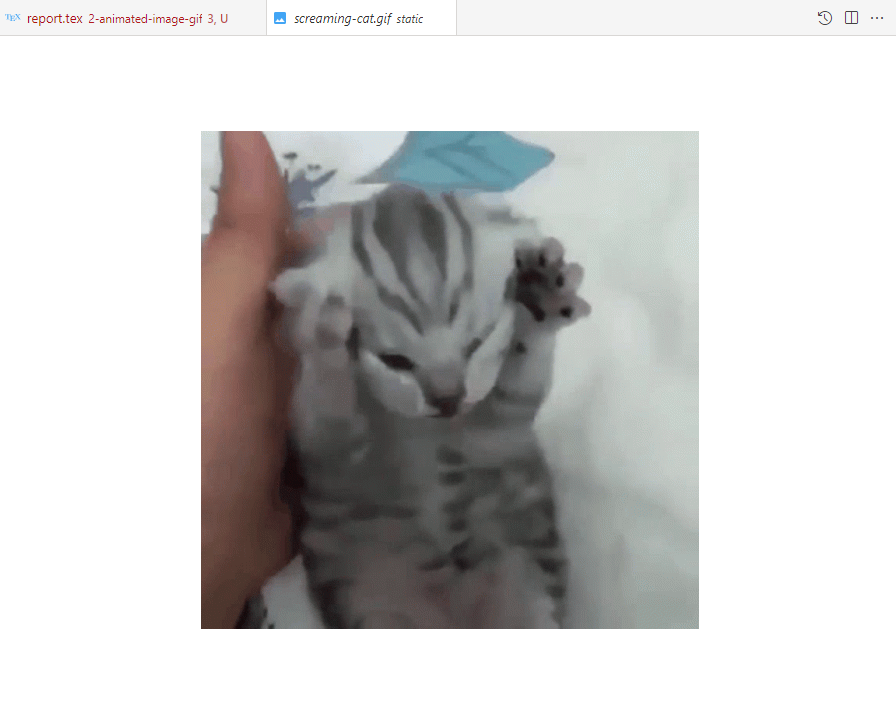
\includegraphics[width=0.5\textwidth]{./static/capture1.png}
    \caption{Gambar bergerak yang akan digunakan}
    \label{fig:gambar1}
    \textbf{Sumber:} \url{https://id.pinterest.com/pin/712553972310325442/}
\end{figure}

\begin{lstlisting}[language=Python ,style=code]
    from PIL import Image
    import os

    IMAGE_PATH = "./static/screaming-cat.gif"

    if __name__ == "__main__":
        gif_image = Image.open(IMAGE_PATH)
\end{lstlisting}

\subsection*{Langkah 2: Mengetahui Jumlah Frame}
\tab Setelah membaca gambar bergerak, langkah selanjutnya adalah mengetahui jumlah frame yang ada pada gambar bergerak tersebut. Dengan mengetahui jumlah frame, kita dapat melakukan ekstraksi frame dari gambar bergerak tersebut dengan melakukan iterasi sebanyak jumlah frame yang ada. Untuk mengetahui jumlah frame, kita dapat menggunakan method \texttt{n\_frames} dari objek \texttt{gif\_image} yang telah kita buat sebelumnya.

\begin{lstlisting}[language=Python ,style=code]
    print(f"Jumlah frame: {gif_image.n_frames}")
\end{lstlisting}

\subsection*{Langkah 3: Ekstraksi Frame}
\tab Setelah mengetahui jumlah frame, langkah selanjutnya adalah melakukan ekstraksi frame dari gambar bergerak tersebut. Untuk melakukan ekstraksi frame, kita dapat menggunakan method \texttt{seek} dari objek \texttt{gif\_image} yang telah kita buat sebelumnya. Method \texttt{seek} ini memungkinkan kita untuk melakukan navigasi ke frame tertentu. Setelah itu, kita dapat menyimpan frame tersebut ke dalam file gambar baru.

\begin{lstlisting}[language=Python ,style=code]
    if not os.path.exists("./static/extracted_frames"):
        os.mkdir("./static/extracted_frames")

    for i in range(gif_image.n_frames):
        gif_image.seek(i)
        frame.save(f"./static/extracted_frames/frame_{i}.png")
\end{lstlisting}

\subsection*{Langkah 4: Merubah Frame}
\tab Setelah melakukan ekstraksi frame, langkah selanjutnya adalah melakukan perubahan pada frame tersebut. Pada praktikum ini, kita akan melakukan perubahan pada frame dengan cara mengubah warna dari frame tersebut. Untuk melakukan perubahan warna, kita dapat menggunakan method \texttt{convert} dari objek \texttt{gif\_image} yang telah kita buat sebelumnya.

\begin{lstlisting}[language=Python ,style=code]
    for i in range(gif_image.n_frames):
        gif_image.seek(i)
        frame = gif_image.convert("L")
        frame.save(f"./static/extracted_frames/frame_{i}.png")
\end{lstlisting}

\begin{figure}[H]
    \centering
    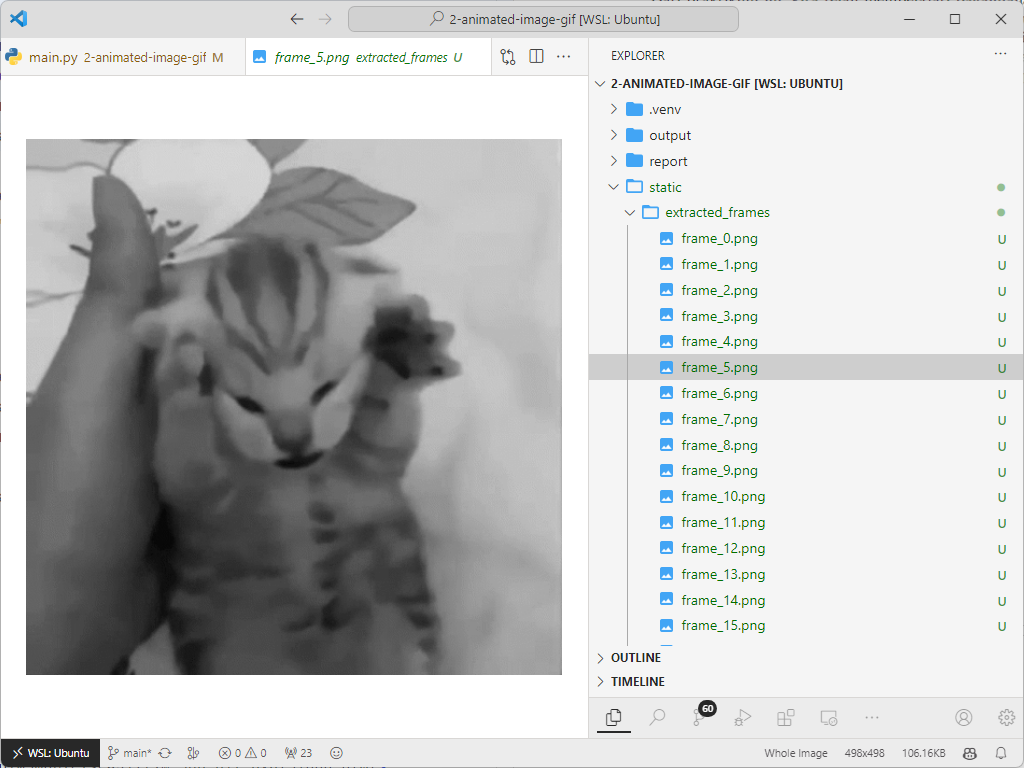
\includegraphics[width=0.5\textwidth]{./static/capture2.png}
    \caption{Frame yang telah diubah warnanya}
    \label{fig:gambar2}
\end{figure}

\subsection*{Langkah 5: Membuat Gambar Bergerak Baru}
\tab Langkah berikutnya adalah menyusun kembali frame-frame tersebut menjadi gambar bergerak baru. Untuk menyusun kembali frame-frame tersebut, kita dapat menggunakan method \texttt{save} dari objek \texttt{gif\_image} yang telah kita buat sebelumnya, dengan menyertakan parameter \texttt{save\_all=True} dan \texttt{append\_images=frames[1:]}. Dengan demikian, kita telah berhasil membuat gambar bergerak baru dari frame-frame yang telah kita ekstraksi sebelumnya berdasarkan gambar bergerak yang telah kita baca sebelumnya.

\begin{lstlisting}[language=Python ,style=code]
    frames[0].save("./static/new_gif.gif", save_all=True, append_images=frames[1:], loop=0, duration=gif_image.info["duration"])
\end{lstlisting}
\begin{figure}[H]
    \centering
    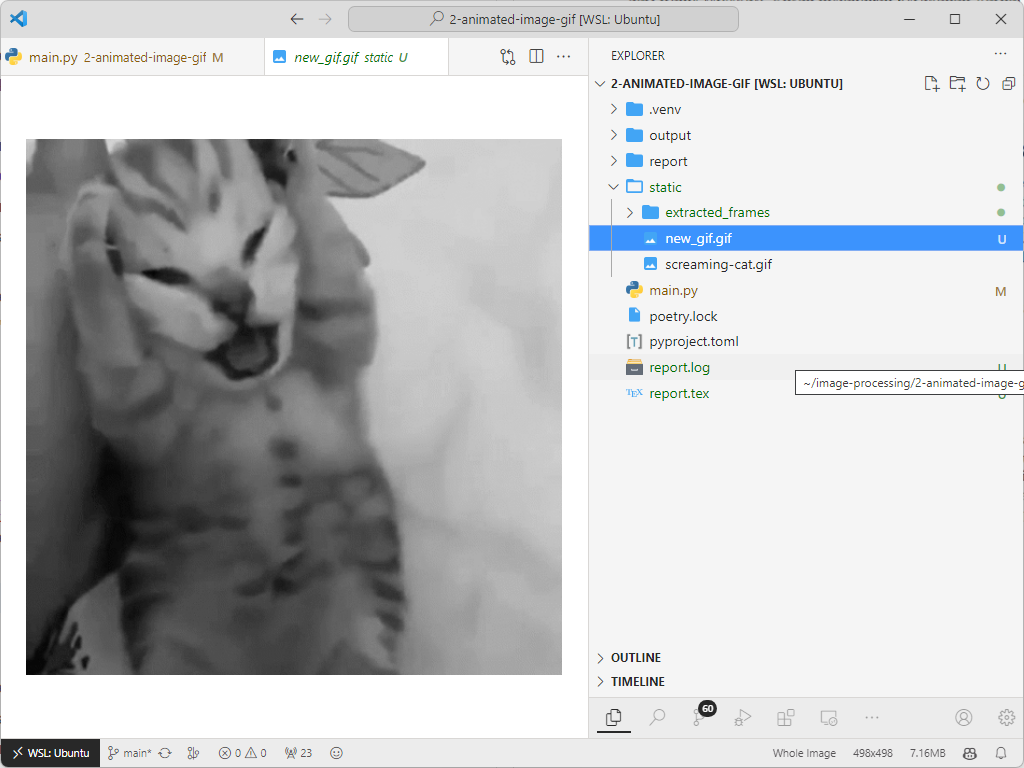
\includegraphics[width=0.5\textwidth]{./static/capture3.png}
    \caption{Gambar bergerak baru yang telah dibuat}
    \label{fig:gambar3}
\end{figure}


\section*{Kesimpulan}
\tab Dari praktikum ini, kita telah mempelajari bagaimana cara melakukan ekstraksi frame dari gambar bergerak, melakukan perubahan pada frame, dan menyusun kembali frame-frame tersebut menjadi gambar bergerak baru. Untuk program lengkapnya, dapat dilihat pada bagian lampiran di akhir laporan ini. Dengan demikian, kita telah memahami konsep dasar pembuatan gambar bergerak dalam format GIF dengan menggunakan bahasa pemrograman Python dan perpustakaan PIL.


\break

\section*{Daftar Pustaka}


\begin{enumerate}
    \item \url{https://www.eecis.udel.edu/~amer/CISC651/lzw.and.gif.explained.html}
    \item \textit{Pillow Documentation}. \url{https://pillow.readthedocs.io/en/stable/}
\end{enumerate}

\break

\section*{Lampiran}
\subsubsection*{Program Lengkap}
\begin{lstlisting}[language=Python ,style=code]
    from PIL import Image
    import os

    IMAGE_PATH = "./static/screaming-cat.gif"

    if not os.path.exists("./static/extracted_frames"):
        os.mkdir("./static/extracted_frames")

    if __name__ == "__main__":
        gif_image = Image.open(IMAGE_PATH)
        print(f"Jumlah frame: {gif_image.n_frames}")
        for i in range(gif_image.n_frames):
            gif_image.seek(i)
            frame = gif_image.convert("L")
            frame.save(f"./static/extracted_frames/frame_{i}.png")
        frames = [Image.open(f"./static/extracted_frames/frame_{i}.png") for i in range(gif_image.n_frames)]
        frames[0].save("./static/new_gif.gif", save_all=True, append_images=frames[1:], loop=0, duration=gif_image.info["duration"])
\end{lstlisting}
\end{document}